\chapter{Time Evolution, Interference, and the Schr\"odinger Equation}

This lecture begins with a short classical reminder and then pivots sharply to the quantum question: how do states change with time? The classical review is not there to reteach mechanics. Its purpose is narrower and more structural. In both classical and quantum physics, the Hamiltonian is the object that generates motion. Starting from that point, we rebuild unitary time evolution, derive the abstract Schr\"odinger equation from an infinitesimal update rule, test it on photon polarization, and then carry the same formalism over to a particle on a line. These notes follow Leonard Susskind's lecture, with supporting board-frame evidence curated by LazyingArt LLC and Video2Book.

\section{From Classical Flow To The Hamiltonian}

Susskind begins with the contrast between discrete and continuous classical systems. A discrete system can hop from one state to another only in sampled time steps. Continuous time becomes natural only when the system itself has continuous degrees of freedom, as for a particle moving on a line. Then the description is no longer a graph of jumps. It is a flow in phase space.

For a particle on a line, the classical state is specified by a position $x$ and a momentum $p$. The Hamiltonian is a function of those variables, and in the simplest nontrivial example it is just kinetic plus potential energy:
\begin{equation}
H(x,p)=\frac{p^2}{2m}+U(x).
\end{equation}
In the lecture frame the equality sign and punctuation are partly obscured, so this printed form should be read as the cautious canonical completion of what is on the board.

\begin{figure}[h]
\centering

\includegraphics[width=0.62\textwidth]{lecture_08_figure_02.png}
\par
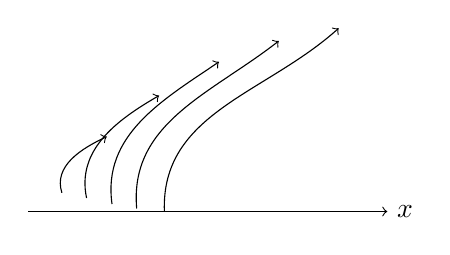
\begin{tikzpicture}[scale=0.95]
\draw[->] (0,0) -- (4.8,0) node[right] {$x$};
\draw[->] (0.45,0.25) to[out=108,in=205] (1.05,1.00);
\draw[->] (0.78,0.18) to[out=102,in=210] (1.75,1.55);
\draw[->] (1.12,0.10) to[out=98,in=214] (2.55,2.00);
\draw[->] (1.45,0.04) to[out=95,in=218] (3.35,2.28);
\draw[->] (1.82,0.00) to[out=92,in=222] (4.15,2.45);
\end{tikzpicture}
\caption{Classical Hamiltonian and flow-line sketch. The TikZ redraw is deliberately schematic: the lecture frame secures the curved flow and the $x$ label, but not a full axis system.}
\end{figure}

The motion is determined by Hamilton's equations,
\begin{align}
\dot x &= \frac{\partial H}{\partial p}, &
\dot p &= -\frac{\partial H}{\partial x}.
\end{align}
Thus for the specific Hamiltonian above, $\partial H/\partial p=p/m$, which is the velocity, and $\partial H/\partial x$ gives the force through the derivative of the potential.

Now if $f(x,p)$ is any classical observable, its time derivative follows from the chain rule:
\begin{align}
\dot f
&= \frac{\partial f}{\partial x}\dot x+\frac{\partial f}{\partial p}\dot p \\
&= \frac{\partial f}{\partial x}\frac{\partial H}{\partial p}
   -\frac{\partial f}{\partial p}\frac{\partial H}{\partial x}.
\end{align}
This combination is the Poisson bracket with the Hamiltonian:
\begin{equation}
\dot f=\{f,H\}_{\mathrm{PB}}.
\end{equation}

The lecture immediately compresses all of this into a single sentence: the Hamiltonian generates time evolution. The detailed Poisson-bracket machinery is less important here than that structural statement. It is precisely that statement which will survive into quantum mechanics.

\section{From Preserved Relations To Unitary Evolution}

Susskind's next move is not to quantize a classical trajectory. It is to ask what quantum mechanics preserves. His answer is that the relations between states do not change with time. Orthogonality stays orthogonality. Inner products stay inner products. One can picture the entire space of states as rotating, while the angles between vectors remain fixed.

If a state $|A\rangle$ evolves for a time $T$, we write
\begin{equation}
|A\rangle \mapsto U(T)|A\rangle.
\end{equation}
Likewise a second state $|B\rangle$ evolves to $U(T)|B\rangle$, and the corresponding bra evolves as
\begin{equation}
\langle B| \mapsto \langle B|U^\dagger(T).
\end{equation}
Preservation of the inner product means
\begin{equation}
\langle B|A\rangle=\langle B|U^\dagger(T)U(T)|A\rangle
\end{equation}
for arbitrary $|A\rangle$ and $|B\rangle$. Therefore
\begin{equation}
U^\dagger(T)U(T)=1.
\end{equation}
So the time-evolution operator is unitary.

This is the clean quantum replacement for classical flow. In classical mechanics we computed how observables change along phase-space trajectories. In quantum mechanics we demand instead that distinctions between states are never erased. From that demand, unitarity follows.

\section{Infinitesimal Time Steps And The Abstract Schr\"odinger Equation}

The next question is local: what is $U(\epsilon)$ for a very short time interval $\epsilon$? Since no evolution at all should do nothing, we must have
\begin{equation}
U(0)=1.
\end{equation}
So for small $\epsilon$ the most general first-order form is
\begin{equation}
U(\epsilon)=1-\frac{i\epsilon}{\hbar}H+O(\epsilon^2).
\end{equation}
At this stage, as Susskind emphasizes, the factors of $i$ and $\hbar$ are partly conventional. They are introduced so that the operator $H$ will later line up with the Hamiltonian, that is, with energy.

Taking the Hermitian conjugate gives
\begin{equation}
U^\dagger(\epsilon)=1+\frac{i\epsilon}{\hbar}H^\dagger+O(\epsilon^2).
\end{equation}
Now impose unitarity to first order:
\begin{align}
1
&=U^\dagger(\epsilon)U(\epsilon) \\
&=\left(1+\frac{i\epsilon}{\hbar}H^\dagger\right)
  \left(1-\frac{i\epsilon}{\hbar}H\right)+O(\epsilon^2) \\
&=1+\frac{i\epsilon}{\hbar}(H^\dagger-H)+O(\epsilon^2).
\end{align}
Therefore the first-order correction must vanish, and we conclude
\begin{equation}
H^\dagger=H.
\end{equation}
The generator of time evolution must be Hermitian.

That already tells us something physical. A Hermitian operator is an observable: it has real eigenvalues and an orthonormal basis of eigenvectors. Only after reaching this point does Susskind give the operator its name. We call it the Hamiltonian, and we call its eigenvalues energies.

Now turn the infinitesimal update into a differential equation. If
\begin{equation}
|\psi(t+\epsilon)\rangle
=
\left(1-\frac{i\epsilon}{\hbar}H\right)|\psi(t)\rangle,
\end{equation}
then
\begin{equation}
\frac{|\psi(t+\epsilon)\rangle-|\psi(t)\rangle}{\epsilon}
=
-\frac{i}{\hbar}H|\psi(t)\rangle.
\end{equation}
Taking the limit $\epsilon\to 0$ gives
\begin{equation}
\frac{\partial}{\partial t}|\psi\rangle=-\frac{i}{\hbar}H|\psi\rangle,
\end{equation}
or, in the canonical form,
\begin{equation}
i\hbar\,\frac{\partial}{\partial t}|\psi\rangle=H|\psi\rangle.
\end{equation}
This is the abstract Schr\"odinger equation. It is not yet the original wave equation Schr\"odinger wrote down for a particle in space. It is the general law of quantum time evolution.

Later in the lecture, after setting $\hbar=1$ temporarily, the same ket equation appears on the board in the simpler form shown below:
\begin{figure}[h]
\centering

\includegraphics[width=0.42\textwidth]{lecture_08_figure_04.png}
\caption{Ket form of the Schr\"odinger equation in the lecture's temporary $\hbar=1$ convention.}
\end{figure}

\section{Polarization Example: Energy Eigenstates And Phase Evolution}

The lecture does not leave the equation abstract for long. Instead it returns to the two-state system of photon polarization. Suppose we have a material in which the $x$ and $y$ polarizations of a photon of fixed wavelength have different energies, say $E_1$ and $E_2$. Then the two basis states are eigenvectors of the Hamiltonian:
\begin{equation}
H|x\rangle=E_1|x\rangle,
\qquad
H|y\rangle=E_2|y\rangle.
\end{equation}

\begin{figure}[h]
\centering

\includegraphics[width=0.74\textwidth]{lecture_08_figure_03.png}
\caption{Polarization energy eigenstates and time-dependent state. The lower state vector is partly blocked in the board frame, so the printed form below follows the transcript.}
\end{figure}

The state of the polarization can be written as a two-component vector,
\begin{equation}
|\psi(t)\rangle=
\begin{pmatrix}
\alpha(t)\\
\beta(t)
\end{pmatrix},
\end{equation}
where $\alpha(t)$ is the amplitude for $x$ polarization and $\beta(t)$ is the amplitude for $y$ polarization.

From this point in the live lecture Susskind suppresses $\hbar$ and works in units with $\hbar=1$. We will keep $\hbar$ in the printed formulas, since that makes the physical dimensions clearer, but the board equations are the same equations with $\hbar$ omitted.

In the $(|x\rangle,|y\rangle)$ basis the Hamiltonian is diagonal:
\begin{equation}
H=
\begin{pmatrix}
E_1 & 0\\
0 & E_2
\end{pmatrix}.
\end{equation}
Here the live lecture briefly writes the diagonal entries in the wrong order and then corrects them; the corrected matrix above is the one to keep.

Applying the Schr\"odinger equation gives
\begin{equation}
i\hbar\frac{d}{dt}
\begin{pmatrix}
\alpha\\
\beta
\end{pmatrix}
=
\begin{pmatrix}
E_1 & 0\\
0 & E_2
\end{pmatrix}
\begin{pmatrix}
\alpha\\
\beta
\end{pmatrix},
\end{equation}
so the two components satisfy separate equations,
\begin{equation}
i\hbar\,\dot\alpha=E_1\alpha,
\qquad
i\hbar\,\dot\beta=E_2\beta.
\end{equation}
These are as simple as they look. Each amplitude changes in time proportionally to itself, so each one picks up a phase:
\begin{equation}
\alpha(t)=\alpha(0)e^{-iE_1 t/\hbar},
\qquad
\beta(t)=\beta(0)e^{-iE_2 t/\hbar}.
\end{equation}
Thus
\begin{equation}
|\psi(t)\rangle=
\begin{pmatrix}
\alpha(0)e^{-iE_1 t/\hbar}\\
\beta(0)e^{-iE_2 t/\hbar}
\end{pmatrix}.
\end{equation}

If we now ask for the probabilities of finding the photon in the $x$ or $y$ basis, nothing seems to happen:
\begin{equation}
|\alpha(t)|^2=|\alpha(0)|^2,
\qquad
|\beta(t)|^2=|\beta(0)|^2.
\end{equation}
At first sight this is almost disappointing. The state evolves, but the obvious probabilities do not.

\subsection{Question \& Answer}

\paragraph{Question.}
If each component only picks up a phase, and if the $x/y$ probabilities do not change, why should we say that anything observable has happened at all?

\paragraph{Answer.}
Because we have asked the wrong measurement question. Phases disappear only when we measure in the same basis in which the Hamiltonian is diagonal. If we rotate the measurement basis, the relative phase becomes visible through interference.

Take the $45^\circ$ polarization state
\begin{equation}
|/\rangle=\frac{1}{\sqrt2}
\begin{pmatrix}
1\\
1
\end{pmatrix}.
\end{equation}
The amplitude that the evolved state passes a $45^\circ$ polarizer is
\begin{equation}
\langle /|\psi(t)\rangle
=
\frac{1}{\sqrt2}
\left(
\alpha(0)e^{-iE_1 t/\hbar}
+
\beta(0)e^{-iE_2 t/\hbar}
\right).
\end{equation}

Now specialize to the case emphasized in the lecture: the photon first passes through a $45^\circ$ polarizer, so initially
\begin{equation}
\alpha(0)=\beta(0)=\frac{1}{\sqrt2}.
\end{equation}
Then the amplitude becomes
\begin{equation}
A_{/}(t)
=
\frac12
\left(
e^{-iE_1 t/\hbar}
+
e^{-iE_2 t/\hbar}
\right).
\end{equation}
The probability is the modulus squared:
\begin{align}
P(t)
&=|A_{/}(t)|^2 \\
&=\frac14
\left(
e^{-iE_1 t/\hbar}+e^{-iE_2 t/\hbar}
\right)
\left(
e^{iE_1 t/\hbar}+e^{iE_2 t/\hbar}
\right) \\
&=\frac14
\left(
2+e^{i(E_2-E_1)t/\hbar}+e^{-i(E_2-E_1)t/\hbar}
\right).
\end{align}
If we define
\begin{equation}
\Delta E=E_2-E_1,
\end{equation}
then
\begin{equation}
P(t)=\frac12\left(1+\cos\frac{\Delta E\,t}{\hbar}\right).
\end{equation}

This is the crucial payoff. The state has not been frozen at all. The relative phase between the two components produces an oscillating transmission probability. At $t=0$, the probability is $1$, exactly as it should be for two parallel polarizers with no time to evolve between them. Later it can fall to $0$, meaning that the photon will certainly fail to pass the second polarizer in the original direction. In the lecture this is interpreted physically as a rotation of the linear polarization as the photon propagates through the material.

The important structural lesson is that only energy differences matter. If we add the same constant to both energies, then both components acquire the same overall phase. That common phase cancels from every probability. The physics depends on $\Delta E$, not on the absolute zero of energy.

\section{Expectation Values, Commutators, And Conserved Quantities}

Having seen in one concrete example that time-dependent phases can have measurable consequences, Susskind steps back and asks for a general rule. Let $K$ be any observable. We want to know how its expectation value
\begin{equation}
\langle K\rangle=\langle\psi|K|\psi\rangle
\end{equation}
changes with time.

\begin{figure}[h]
\centering

\includegraphics[width=0.62\textwidth]{lecture_08_figure_05.png}
\caption{Product-rule step toward the commutator formula. The visible board line secures the structure of the derivation, while the full printed equation below is reconstructed from the transcript.}
\end{figure}

The first step is just the product rule:
\begin{equation}
\frac{d}{dt}\langle\psi|K|\psi\rangle
=
\langle\psi|K|\dot\psi\rangle
+
\langle\dot\psi|K|\psi\rangle.
\end{equation}
Now use the Schr\"odinger equation for the ket and its Hermitian conjugate for the bra:
\begin{equation}
|\dot\psi\rangle=-\frac{i}{\hbar}H|\psi\rangle,
\qquad
\langle\dot\psi|=\frac{i}{\hbar}\langle\psi|H.
\end{equation}
Substituting these into the product rule gives
\begin{align}
\frac{d}{dt}\langle K\rangle
&=
\left\langle\psi\left|K\left(-\frac{i}{\hbar}H\right)\right|\psi\right\rangle
+
\left\langle\psi\left|\left(\frac{i}{\hbar}H\right)K\right|\psi\right\rangle \\
&=
-\frac{i}{\hbar}\langle\psi|KH|\psi\rangle
+\frac{i}{\hbar}\langle\psi|HK|\psi\rangle \\
&=
-\frac{i}{\hbar}\langle\psi|(KH-HK)|\psi\rangle.
\end{align}
With the convention
\begin{equation}
[K,H]=KH-HK,
\end{equation}
the time-evolution law becomes
\begin{equation}
\frac{d}{dt}\langle K\rangle
=
-\frac{i}{\hbar}\langle[K,H]\rangle.
\end{equation}
The live lecture briefly wavers between commutator orders and signs, but this is the clean convention consistent with the algebra just written.

This is the quantum analog of the classical statement $\dot f=\{f,H\}_{\mathrm{PB}}$. In both theories, the Hamiltonian is the thing that tells us how observables change with time. Only the bracket has changed.

\begin{proposition}
If an observable $K$ commutes with the Hamiltonian, then its expectation value is conserved:
\begin{equation}
[K,H]=0
\qquad \Longrightarrow \qquad
\frac{d}{dt}\langle K\rangle=0.
\end{equation}
\end{proposition}

\begin{proof}
If $[K,H]=0$, then the right-hand side of
\[
\frac{d}{dt}\langle K\rangle=-\frac{i}{\hbar}\langle[K,H]\rangle
\]
vanishes identically.
\end{proof}

Susskind remarks that one can prove a stronger theorem about the full probability distribution, but for the moment the expectation-value statement is enough. In particular, the Hamiltonian commutes with itself, so the Hamiltonian is conserved. Since the Hamiltonian is the energy, energy conservation drops straight out of the formalism.

\section{Particle On A Line And The Free-Particle Schr\"odinger Equation}

The lecture closes by translating the abstract operator story into the language of wave functions. For a particle on a line, the state vector can be represented by a wave function $\psi(x,t)$. One may equally well work in momentum space with the Fourier transform $\tilde\psi(p,t)$, but the position-space form is the natural one for writing the original Schr\"odinger equation.

The rule of time evolution is the same as before:
\begin{equation}
i\hbar\,\frac{\partial}{\partial t}\psi(x,t)=H\psi(x,t).
\end{equation}
What is different is only the concrete form of the Hamiltonian.

For a free particle with no forces, the classical energy is
\begin{equation}
E=\frac{p^2}{2m}.
\end{equation}
This does not prove the quantum Hamiltonian, but it strongly suggests the guess
\begin{equation}
\hat H=\frac{\hat p^2}{2m}.
\end{equation}
With
\begin{equation}
\hat p=-i\hbar\frac{\partial}{\partial x},
\end{equation}
we find
\begin{equation}
\hat H
=
\frac{1}{2m}
\left(-i\hbar\frac{\partial}{\partial x}\right)^2
=
-\frac{\hbar^2}{2m}\frac{\partial^2}{\partial x^2}.
\end{equation}
In the live lecture Susskind pauses here, notices missing factors and sign confusion, and then redoes the calculation carefully. The cleaned final result is the one above.

Therefore the free-particle Schr\"odinger equation is
\begin{equation}
i\hbar\,\frac{\partial}{\partial t}\psi(x,t)
=
-\frac{\hbar^2}{2m}\frac{\partial^2}{\partial x^2}\psi(x,t).
\end{equation}

\paragraph{A worked solution.}
Look for a solution that is an eigenfunction of momentum at every instant:
\begin{equation}
\psi_p(x,t)=f(t)e^{ipx/\hbar}.
\end{equation}
The time derivative hits only $f(t)$:
\begin{equation}
\frac{\partial \psi_p}{\partial t}
=
\dot f(t)e^{ipx/\hbar}.
\end{equation}
The second spatial derivative hits only the exponential:
\begin{equation}
\frac{\partial^2 \psi_p}{\partial x^2}
=
-\frac{p^2}{\hbar^2}f(t)e^{ipx/\hbar}.
\end{equation}
Substituting into the Schr\"odinger equation gives
\begin{equation}
i\hbar\,\dot f(t)e^{ipx/\hbar}
=
\frac{p^2}{2m}f(t)e^{ipx/\hbar}.
\end{equation}
Cancel the common spatial factor to obtain
\begin{equation}
i\hbar\,\dot f=\frac{p^2}{2m}f,
\qquad\text{or}\qquad
\dot f=-\frac{i p^2}{2m\hbar}f.
\end{equation}
Hence
\begin{equation}
f(t)=e^{-ip^2 t/(2m\hbar)}
\end{equation}
up to an overall constant, and the full solution is
\begin{equation}
\psi_p(x,t)
=
\exp\!\left[\frac{i}{\hbar}\left(px-\frac{p^2}{2m}t\right)\right]
\end{equation}
up to normalization.

Again the time dependence is a pure phase. For a single momentum eigenstate, the state does not change its character; it only accumulates the phase appropriate to its energy. The lecture closes by pointing out the simple exercise
\begin{equation}
[p,H]=0
\qquad\text{for}\qquad
H=\frac{p^2}{2m},
\end{equation}
so momentum is conserved for the free particle.

\section{Summary}

The chapter has followed the lecture's basic arc. We began with classical flow only long enough to isolate the structural role of the Hamiltonian. In quantum mechanics that role becomes sharper: preservation of inner products leads to unitary evolution, infinitesimal unitarity forces the generator to be Hermitian, and the infinitesimal update rule becomes the Schr\"odinger equation.

The polarization example then shows what the formalism means. A Hamiltonian diagonal in the $x/y$ basis gives each component its own phase. Those phases look invisible until we measure in another basis, where they interfere and produce oscillating probabilities controlled only by energy differences. From there the commutator law for expectation values follows almost immediately, and the same machinery carries over to a particle on a line, where it becomes the familiar free-particle Schr\"odinger equation.